\documentclass[12pt,a4paper,ngerman]{article}

\usepackage[utf8]{inputenc} % set input encoding (not needed with XeLaTeX)
\usepackage[ngerman, num]{isodate}
\usepackage[ngerman]{babel}
\usepackage[]{hyperref}
\usepackage[table]{xcolor}
\usepackage{graphicx}
\usepackage{geometry} % to change the page dimensions
\geometry{a4paper} % or letterpaper (US) or a5paper or....

% \usepackage[parfill]{parskip} % Activate to begin paragraphs with an empty line rather than an indent


\title{Detailspezifikation IPOM}
%\author{The Author}
%\date{} % Activate to display a given date or no date (if empty),
         % otherwise the current date is printed

\begin{document}
\maketitle
\tableofcontents

\section{Reqs}
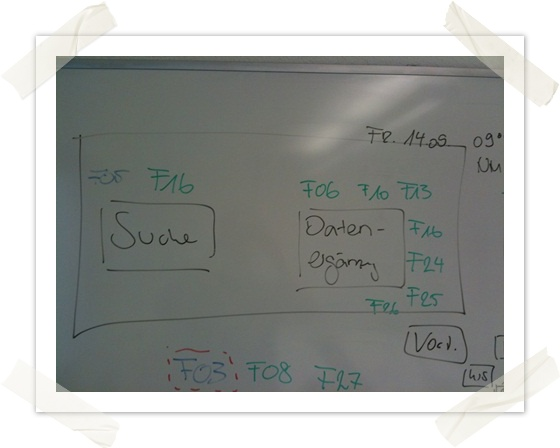
\includegraphics[width=15cm]{WS+1.JPG}
#foreach ($issue in $jq.project('').children(''))
    \subsection{$issue.summary} \label{$issue.key}
    $issue.description
#end

\end{document}
